%% Based on a TeXnicCenter-Template by Tino Weinkauf.
%%%%%%%%%%%%%%%%%%%%%%%%%%%%%%%%%%%%%%%%%%%%%%%%%%%%%%%%%%%%%

%%%%%%%%%%%%%%%%%%%%%%%%%%%%%%%%%%%%%%%%%%%%%%%%%%%%%%%%%%%%%
%% HEADER
%%%%%%%%%%%%%%%%%%%%%%%%%%%%%%%%%%%%%%%%%%%%%%%%%%%%%%%%%%%%%
\documentclass[a4paper,10pt]{article}

% Alternative Options:
%	Paper Size: a4paper / a5paper / b5paper / letterpaper / legalpaper / executivepaper
% Duplex: oneside / twoside
% Base Font Size: 10pt / 11pt / 12pt

\usepackage[spanish]{babel}  	% Traduce los textos a castellano
\usepackage[utf8]{inputenc}	% Permite escribir directamente áéíóúñ
\usepackage{t1enc}            	% Agrega caracteres extendidos al font
\usepackage{amsmath} 		%Permite imprimir mas opcciones matematicas
\usepackage{graphicx}		%Permite agregar imagenes al informe
\usepackage{multicol}  		%Permite dividir el texto en varias columnas
\usepackage{anysize}		%Permite modificar los margenes del documento
\usepackage{float} 		%Permite utilizar H para colocar las imagenes en un lugar especifico 
\usepackage{multirow}		%Permite dividir las tablas en subtablas
\usepackage{booktabs}		%Permiten manejar mejor el tamaño de las tablas
\usepackage{tabulary}		%Permiten manejar mejor el tamaño de las tablas
\usepackage{fancyhdr}		%Permite agregar encabezado y pie fancy


%% Packages for Graphics & Figures %%%%%%%%%%%%%%%%%%%%%%%%%%
\usepackage{graphicx} %%For loading graphic files
%\usepackage{subfig} %%Subfigures inside a figure
%\usepackage{pst-all} %%PSTricks - not useable with pdfLaTeX

%% Please note:
%% Images can be included using \includegraphics{Dateiname}
%% resp. using the dialog in the Insert menu.
%% 
%% The mode "LaTeX => PDF" allows the following formats:
%%   .jpg  .png  .pdf  .mps
%% 
%% The modes "LaTeX => DVI", "LaTeX => PS" und "LaTeX => PS => PDF"
%% allow the following formats:
%%   .eps  .ps  .bmp  .pict  .pntg


%% Math Packages %%%%%%%%%%%%%%%%%%%%%%%%%%%%%%%%%%%%%%%%%%%%
\usepackage{amsmath}
\usepackage{amsthm}
\usepackage{amsfonts}



%% Line Spacing %%%%%%%%%%%%%%%%%%%%%%%%%%%%%%%%%%%%%%%%%%%%%
%\usepackage{setspace}
%\singlespacing        %% 1-spacing (default)
%\onehalfspacing       %% 1,5-spacing
%\doublespacing        %% 2-spacing

\usepackage{fancyhdr}
\setlength{\headheight}{13pt} 

%% Other Packages %%%%%%%%%%%%%%%%%%%%%%%%%%%%%%%%%%%%%%%%%%%
\usepackage{a4wide} %%Smaller margins = more text per page.
%\usepackage{fancyhdr} %%Fancy headings
%\usepackage{longtable} %%For tables, that exceed one page


%%%%%%%%%%%%%%%%%%%%%%%%%%%%%%%%%%%%%%%%%%%%%%%%%%%%%%%%%%%%%
%% Remarks
%%%%%%%%%%%%%%%%%%%%%%%%%%%%%%%%%%%%%%%%%%%%%%%%%%%%%%%%%%%%%
%
% TODO:
% 1. Edit the used packages and their options (see above).
% 2. If you want, add a BibTeX-File to the project
%    (e.g., 'literature.bib').
% 3. Happy TeXing!
%
%%%%%%%%%%%%%%%%%%%%%%%%%%%%%%%%%%%%%%%%%%%%%%%%%%%%%%%%%%%%%

%%%%%%%%%%%%%%%%%%%%%%%%%%%%%%%%%%%%%%%%%%%%%%%%%%%%%%%%%%%%%
%% Options / Modifications
%%%%%%%%%%%%%%%%%%%%%%%%%%%%%%%%%%%%%%%%%%%%%%%%%%%%%%%%%%%%%

%\input{options} %You need a file 'options.tex' for this
%% ==> TeXnicCenter supplies some possible option files
%% ==> with its templates (File | New from Template...).



%%%%%%%%%%%%%%%%%%%%%%%%%%%%%%%%%%%%%%%%%%%%%%%%%%%%%%%%%%%%%
%% DOCUMENT
%%%%%%%%%%%%%%%%%%%%%%%%%%%%%%%%%%%%%%%%%%%%%%%%%%%%%%%%%%%%%
\begin{document}
%
% Hago que en la cabecera de página se muestre a la derecha la sección,
% y en el pie, en número de página a la derecha:
%
\pagestyle{fancy}
\renewcommand{\sectionmark}[1]{\markboth{}{\thesection\ \ #1}}
\lhead{}
\chead{}
\rhead{\rightmark}
\lfoot{}
\cfoot{}
\rfoot{\thepage}

%% Title Page %%%%%%%%%%%%%%%%%%%%%%%%%%%%%%%%%%%%%%%%%%%%%%%
%% ==> Write your text here or include other files.

%
% Carátula:
%

\author{Firstname Lastname}
%\date{} %%If commented, the current date is used.

\begin{titlepage}

\thispagestyle{empty}
\begin{center}
\includegraphics[scale=0.2]{Imagenes/FIUBA_ALTA.jpg}\\
\large{\textsc{Universidad de Buenos Aires}}\\
\large{\textsc{Facultad De Ingeniería}}\\
\small{Año 2015 - 2\textsuperscript{do} Cuatrimestre}\\
\vspace{1cm}
\Large{\underline{\textsc{Taller de Desarrollo de Proyectos (75.45)}}}
\end{center}



%% The simple version:
\title{Sistema de Consultas Médicas Dr. Me.}

\begin{center}
\Large{\textit{\bf{Sistema de Consultas Médicas}}}\\
\Large{\textit{\bf{Dr. Me}}}\\
\textit{\bf{Modelo comercial}}
\end{center}

\vspace{1cm}

\raggedright{\Large{\textit{\bf{Integrantes}}}}

\vspace{0.5cm}

\begin{center}
  Julián Scialabba,	\textit{P. 00.000},	\textit{julian.scialabba@gmail.com}		\\
  Facundo Rossi,		\textit{P. 00.000},	\textit{frossi85@gmail.com}		\\
  Débora Martin,		\textit{P. 00.000},	\textit{debbie1new.world@gmail.com}	\\
  Matías Manzano,			\textit{P. 00.000},	\textit{matsebman@gmail.com}		\\
  Ariel Barreiro,		\textit{P. 00.000},	\textit{damian168@gmail.com}		\\
  Sebastian Rial,			\textit{P. 00.000},	\textit{aberrei@gmail.com}		\\
\end{center}

\end{titlepage}

%
% Hago que las páginas se comiencen a contar a partir de aquí:
%

\setcounter{page}{1}

%
% Pongo el índice en una página aparte:
%

\newpage
\tableofcontents

\newpage
\section{Objetivo}

El objetivo de este proyecto es realizar un sistema que permita a cualquier persona registrada en el mismo, obtener 
un simple diagnóstico aproximado a partir de los síntomas que tal persona presenta, y darle opciones de obtener un turno médico acorde en forma automática y de acuerdo a sus preferencias.

\section{Visión}

Mejorar la salud y la calidad de vida de todas las personas en el mundo.

\section{Misión}

Crear aplicaciones que faciliten las consultas y diagnósticos médicos, disminuyendo tiempos de espera y retrasos.  

Aumentar la certeza y confiabilidad de los diagnósticos automatizados, así como la confianza de las personas en los mismos. 

Continuar mejorando la base de conocimientos médicos con el fin de ampliar el espectro de afecciones abarcados. 

\section{Funcionalidades provistas}

\begin{itemize}
\item Diagnóstico inicial a partir de síntomas ingresados y consecuente derivación a un especialista.
\item Obtención de turnos de acuerdo a diversos filtros (zona, tiempo de espera, médico, obra social o prepaga, centro de salud).
\item Cancelación o modificación de turnos por parte de médico y paciente.
\item Retroalimentación para mejorar la calidad del diagnóstico en base a la experiencia de los usuarios.
\item Historia clínica del paciente online visible al especialista.
\item Recordatorio de próximos turnos.
\item Alertas de retrazo en turnos por parte del médico hacia los pacientes o del paaciente hacia el médico mediante el uso de geoposicionamiento.
\item Recordatorios al paciente sobre controles necesarios o tiempo pasado desde el último control.
\item Posibilidad de evaluar al profesional y al paciente reflejado en un sistema de reputación.
\item Almacenamiento de estadísticas de consultas realizadas y su seguimiento.
\end{itemize}

\section{Modelo de negocio}

La adquisicion del sistema es gratuita para todo tipo de usuarios, sean estos pacientes, médicos o instituciones de salud. Sin embargo, para que el mismo sea rentable, se cuenta con diversos métodos de financiamiento.

\begin{itemize}
\item Por cada turno reservado por este medio y que no haya sido cancelado posteriormente, se cobrará un pequeño monto a la institución o al médico privado.
\item Se venderá espacio para publicidad que será mostrada tanto al paciente como al médico. Dicha publicidad estará principalmente orientada al cuidado de la salud con productos como medicamentos, laboratorios u otros servicios médicos.
\item Dado que se almacenarán estadisticas producto del uso dado por los usuarios al sistema, se ofrecerán estos datos a empresas, como laboratorios o prepagas, que puedan estar interesadas en obtenerlos.
\end{itemize}


\section{Análisis de mercado}

\subsection{Producto}

El sistema que se ofrece es en parte una central de turnos global, que administre todas las obras sociales y prepagas, que siga las preferencias del usuario. Por otro lado, cuenta con un módulo de diagnósticos que analiza los síntomas ingresados por el usuario y devuelve un resultado probable. El conjunto de estos servicios tiene como objetivo minimizar la cantidad de tiempo entre el pedido del turno y el inicio del tratamiento. De esta manera, ante un síntoma no será necesario esperar meses para lograr una primera consulta con un médico clínico y luego iniciar los correspondientes exámenes.

En el caso de los prestadores de los servicios de salud, les permitirá  mejorar la distribución y cantidad de turnos. Además, ofrecerá la posibilidad de que el paciente pueda consultar su diagnóstico y derivarlo al especialista correspondiente, disminuyendo la carga de consultas y la deserción debida a la impaciencia en la primera etapa del tratamiento. No reemplaza completamente al médico clínico ya que se requeriría de su aprobación o su diagnóstico, en ciertos casos en que este no se pueda realizar con cierto grado de certeza. El sistema se retroalimentará con los diagnósticos finales para ir mejorando su efectividad.


\subsection{Precio}

El uso del sistema no se cobrará a los pacientes, ni se cobrará la instalación a los servicios de salud. Sólo se cobrará un pequeña comisión por cada turno reservado por este medio y que no haya sido
cancelado. De cada una de estas consultas tomaremos un $5\%$ de su valor. 

El promedio de la consulta a médico clínico es de $\$200$ por lo que tendríamos $\$10$ de ingreso por consulta. Según la encuesta realizada, el $95\%$ de las personas estaría dispuesta a pagar este monto. Además, se cobraría en caso de ser necesario el soporte técnico de acuerdo a los valores de mercado presentes en ese momento. 

Sin embargo, una de las mayores fuentes de ingreso será la publicidad dirigida a los pacientes y médicos promocionando productos relacionados con la salud, tales como medicamentos, laboratorios, farmacias, prepagas o médicos particulares. El valor se adecuará a los precios del momento para publicidad en internet.

\subsection{Promoción}

La publicidad se realizará mediante las redes sociales para llegar a los pacientes, o por medio de la comunicación directa via mail o personalmente con los prestadores de servicios e instituciones relacionadas.

Estos anuncios en medios masivos tales como Facebook pueden llegar a una gran cantidad de personas en poco tiempo, pero son costosos. Según estadísticas de la red en CABA y Buenos Aires, un $75\%$ de los habitantes alfabetizados utilizan internet casi todos los días. La tasa de alfabetización en Buenos Aires es de $98.7\%$, por lo que la cantidad de personas que utilizan internet regularmente es de $74\%$. El costo de la publicidad depende directamente de la cantidad de gente que la vea. Considerando los datos provistos por la red social Facebook para Argentina, por la inversión en dolares se triplica el número de instalaciones de la aplicación. Además, la cantidad de personas que clickearán en la publicidad será de 15 veces la inversión hecha.

\subsection{Plaza}

Al comienzo del proyecto nos centraremos en la población de CABA y Provincia de Buenos Aires, la cual totaliza unos 14.391.538 habitantes. Aproximadamente 8.3 millones tienen algún tipo de obra social, 2.2 millones utilizan algún tipo de medicina prepaga, y el resto se atiende mediante el sistema público. 

\begin{center}
\begin{figure}[H]
\centering
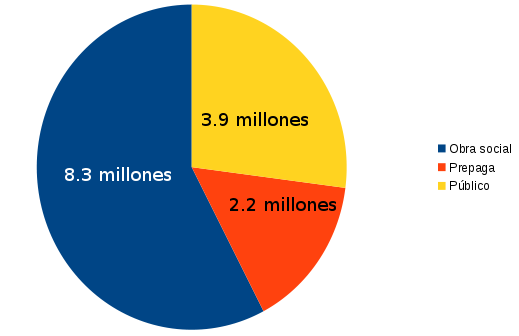
\includegraphics[width=1\textwidth]{./Imagenes/g1.png}
\caption{Distribución de habitantes según cobertura (BA y CABA)}
\label{fig:hp}
\end{figure}
\end{center}

La cantidad de consultas médicas anuales en el sistema privado se estima en un total de 105.8 millones y en 71 millones en el sector público. Podemos realizar una estimación de la aceptación que tendría nuestro sistema considerando que un $2\%$ de estas consultas se efectúan por este medio.

\begin{table} [H]
\begin{center}
\begin{tabular}{|c|c|c|c|}
\hline
		&Consultas anuales (millones)	&Consultas en sistema (millones)	&Ingresos (millones en \$)\\\hline
Privado	&105.8							&2.116								&21.16\\\hline
Público	&71								&1.42								&14.2\\\hline
Total	&176.8							&3.526								&35.26\\\hline
\end{tabular}
\end{center}
\caption{Ingresos estimados por consultas en sistema}
\end{table}

Considerando los proveedores de servicios de salud se encontró que la cantidad de médicos en CABA y Buenos Aires es de unos 57500. Hay además, 4600 establecimientos privados y 300 obras sociales. Suponiendo que un $5\%$ de estos además requieran datos estadísticos en forma anual para distintos fines, como investigaciones científicas, se obtendrían unas 245 solicitudes.

\subsection{Clientes}

\subsubsection{Módulo de turnos}

Los pacientes, que serán la mayoría de los usuarios, se ven beneficiados por la política de centralizar otorgamiento de turnos en forma online, la rapidez y simplicidad del sistema, permitiendo ahorrar tiempo en esperas y en consultas. De acuerdo a la encuesta realizada, el $65\%$ de los interrogados estaría dispuesto a usar este tipo de tecnología y solo el $10\%$ del total no estaría dipuesto a abonar una pequeña cuota mensual. 

Por otro lado, las clínicas y médicos particulares obtendrían un gran beneficio de este sistema porque permite la reorganización de turnos en base a tiempos estándares de consulta y demoras imputables al paciente. Esto ahorraría parte del costo de los turnos perdidos. La antedicha encuesta también revelo que el $95\%$ de las personas están de acuerdo con la digitalización de su historia clínica para obtener acceso instantaneo a la misma.

Según la encuesta realizada por MedicalEconomics, un $55\%$ de los médicos utiliza sistemas electrónicos para los registros de historiales clínicos. Dichos sistemas que solo obtienen la información instantaneamente si se ha realizado el estudio dentro del mismo centro de salud o prepaga. A diferencia de estos, la aplicación que ofrecemos permite no solo el almacenamiento de dicha información, sino la obtención  en tiempo real de cualquier estudio cualquiera sea el lugar que se realice. En principio para este $55\%$ resultaría muy apropiada la utilización de nuestro sistema. De esta porción de médicos, un $60\%$ utiliza servicios basados en la "nube". Para este grupo la adaptación al nuevo sistema no representaría grandes cambios en cuanto a dificultad, obteniendo remarcables beneficios.

Considerando estos valores, podemos estimar que un $30\%$ de los médicos que conozcan la aplicación podrían utilizarla. 

\subsubsection{Módulo de diagnósticos}

El módulo de diagnósticos podría ser quizás el más controvertido de todos debido a que está reemplazando en parte la labor de un profesional. Sin embargo, como se mostrará a continuación podría tener una gran aceptación debido en parte a la saturación del sistema de salud y a la necesidad de agilizar los tiempos de diagnóstico y tratamiento.

Según la encuesta realizada por JMIR publications, el $95\%$ de los médicos y el  $81\%$ de los pacientes cree que la tecnología informática debe utilizarse en la medicina, o se encuentra entusiasmado por su posible uso.

Por otro lado, al $58\%$ de los médicos le gusta la tecnología, pero prefiere los diagnósticos profesionales, mientras que un $13.8\%$ recomendaria utilizarla para diagnósticos. Solo el $28\%$ se siente incómodo sobre la posible utilización de la misma. En el caso de los pacientes, los resultados son $44.6\%$, $39.66\%$ y $15.88\%$ respectivamente. El porcentaje de profesionales que prefieren el método tradicional sería factible de ser persuadido a reveer su posición al ver los buenos resultados del módulo de diagnósticos. Quizás su indecisión se deba al temor a ser desplazados de su posición y ser reemplazados por este tipo de sistemas. Por lo cual sería necesario hacer incapié en la imposibilidad de dicha supocisión.

\begin{center}
\begin{figure}[H]
\centering
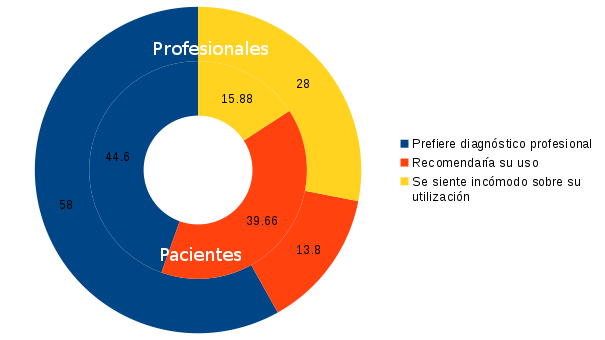
\includegraphics[width=1\textwidth]{./Imagenes/g2.png}
\caption{Reacción de pacientes y profesionales ante la posibilidad de usar diagnostico automatizado (JMIR)}
\label{fig:hp}
\end{figure}
\end{center}


Finalmente, según encuesta de Medscape, se observó que un $69\%$ de los médicos utilizarían la tecnología como ayuda en los diagnósticos, mientras que este porcentaje es de $84\%$ para los pacientes. Además, al menos un $64\%$ de pacientes y un $63\%$ de médicos están de acuerdo en el uso de tecnología, para la realización de estudios clínicos.

\begin{table} [H]
\begin{center}
\begin{tabular}{|c|c|c|c|c|c|}
\hline
			&JMIR 1 (\%)	&JMIR 2 (\%)	&Medscape 1 (\%)	&Medscape 2 (\%)	&Promedio (\%)\\\hline
Médicos		&95							&13.8						&69							&63									&59\\\hline
Pacientes	&81							&15.88						&84							&64									&67\\\hline
\end{tabular}
\end{center}
\caption{Porcentaje de clientes que utilizarían el sistema para diagnósticos}
\end{table}

\subsubsection{Módulo de estadísticas}

Según el Austrian Journal of Statistics, al menos el $75\%$ de los 
papers de medicina utilizan análisis estadísticos para llegar a sus conclusiones. Además, permitirá conocer la cantidad y tipo de pacientes que contraen determinada enfermedad, el tipo de tratamiento que se les aplica y los resultados de determinadas drogas. Por lo que se puede concluir que sería de utilidad para todo ambito de la salud, tanto científico como comercial.

\subsection{Competidores}

Si bien algunas prepagas u hospitales tienen sistemas de turnos online, 
el hecho de que se ofrezcan sus servicios les permitiría captar nuevos clientes particulares, mediante la oferta que muestran. Además, la aplicación ofrece servicios de reacomodamiento de turnos en tiempo real dependiendo del geoposicionamiento del paciente o las actualizaciones de último momento que este realice. Dichos servicios no se encuentran en ninguna aplicación similar y permiten ahorrar parte de las perdidas generadas por estos inconvenientes. Dichas pérdidas se estiman en 
6.01 millones de pesos anuales.

\subsection{Colaboradores}

El sistema brindará la posibilidad de que los usuarios puedan enviar sugerencias, las cuales se evaluarán para ser implementadas. Se pedirá también su colaboración para mantener una base de datos actualizada y eficiente. 
Dado que el beneficio para los prestadores de servicios de salud es amplio, se buscará la ayuda de instituciones como la Asociación de Médicos Argentinos con el fin de publicitar y expandir el sistema.

\subsection{Contexto}

El proyecto quizás podría encontrar algunos inconvenientes iniciales debido a la resistencia al cambio o la posible falta de confianza en las personas. Sin embargo, dado que el mundo en general se encamina en esta dirección, la adopción de este  tipo de tecnologías por parte de los usuarios es prácticamente un hecho. 

Así se puede deducir de articulos donde se considera la posibilidad de introducir los diagnósticos automatizados  \cite{link9}. Otros comentan los diagnósticos que se están realizando con cantidades masivas de datos en supercomputadoras \cite{link10}, o pronostican que el $80\%$ del trabajo que hoy realizan los médicos será realizado en forma digital \cite{link11}.



\section{Conclusiones}

Considerando los datos anteriormente presentados podemos concluir que las ganancias obtenidas por la distribución de este sistema corresponderán aproximadamente con los presentados a continuación.

\begin{equation}
\label{eq:diag_personas}
G_{dp} = 3 X * 0.67 * G_r
\end{equation}

\begin{equation}
\label{eq:diag_medicos}
G_{dm} = 3 X * 0.59 * 0.005 * G_r 
\end{equation}

\begin{equation}
\label{eq:tur_pacientes}
G_{tp} = 3 X * 0.67 * G_r
\end{equation}

\begin{equation}
\label{eq:tur_medicos}
G_{tm} = 3 X * 0.3 * 0.005 * G_r + P_r * C_m * 0.3
\end{equation}

En donde:
\begin{description}
\item[$G_r$]: Factor de crecimiento (tomado de métrica promedio).
\item[$C_m$]: Cantidad total de médicos particulares, clínicas y hospitales. 
\item[$P_r$]: Porcentaje del total de médicos particulares y clínicas a los cuales les presentaremos el sistema personalmente. Supondremos que es del $10\%$.
\item[$G_{dp}$]: Ganancia para el módulo de diagnóstico por parte de los pacientes.
\item[$G_{dm}$]: Ganancia para el módulo de diagnóstico por parte de los prestadores de servicios de salud.
\item[$G_{tp}$]: Ganancia para el módulo de turnos por parte de los pacientes.
\item[$G_{tm}$]: Ganancia para el módulo de turnos por parte de los prestadores de servicios de salud.
\end{description}
 
Debido a que se trata de un proyecto novedoso y no existen datos precisos se hizo una estimación de acuerdo a los datos proporcionados por otras aplicaciones. De acuerdo a esto, la cantidad de gente alcanzada en el primer año sería, con  un factor de crecimiento del $10\%$ mensual y un monto destinado a publicidad de $U\$S 10000$:

\begin{itemize}  
\item Estimación de uso de la aplicación de diagnosticos (pacientes) en el primer año: 63000 usuarios.
\item Estimación de uso de la aplicación de diagnósticos (medicos) primer año: 93 usuarios.
\item Estimación de uso de la aplicación de turnos (pacientes) primer año: 63000 usuarios.
\item Estimación de uso de la aplicación de turnos (servicios de salud)  primer año: 195 usuarios. 
\end{itemize}

Considerando que los 63000 pacientes solicitan unos 170000 turnos, y que cobramos $\$ 10$ por cada una, el ingreso en el primer año, entonces sería de $\$ 1.700.000$. A esto habría que sumarle los ingresos por publicidad y los correspondientes a las ventas realizadas de la base de datos estadística.

Por lo tanto, consideramos que el sistema será no solo rentable, sino que es una buena inversión considerando las proyecciones en materia tecnológica para el ámbito de la salud.

\begin{thebibliography}{23}%El numero es fijo según el numero de referencias
\bibitem{link1} http://www.deis.gov.ar/guia.htm 
\bibitem{link2} https://sisa.msal.gov.ar/sisa/\#sisa 
\bibitem{link3} http://www.ms.gba.gov.ar/wp-content/uploads/2013/04/guia-establecimientos.pdf
\bibitem{link4} http://www.ieps.com.ar/es/template.php?file=notas/2011/11/11\_11\_03\_El-gasto-salud-en-Argentina.html
\bibitem{link5} http://www.keymarket.com.ar/medicina-prepaga.htm
\bibitem{link6} http://www.clarin.com/empresas\_y\_negocios/Salud-privada-sociales-medicina-Argentina\_0\_296370635.html
\bibitem{link7} http://www.deis.msal.gov.ar/publicaciones/archivos/indicadores\_2014.pdf 
\bibitem{link8} http://www.deis.gov.ar/publicaciones/archivos/serie12nro5.pdf 
\bibitem{mag1} Austrian Journal of Statistics, Volume 36, 2007.
\bibitem{link9} https://lifedoctoring.wordpress.com/automated-diagnosis-and-the-future-of-biomedicine/
\bibitem{link10} http://searchhealthit.techtarget.com/feature/Automated-diagnostics-How-supercomputers-fit-in-radiologys-future
\bibitem{link11} http://fortune.com/2012/12/04/technology-will-replace-80-of-what-doctors-do/
\bibitem{link12} http://blog.startupcompass.co/how-to-avoid-74-percent-of-startup-failures-benchmark-growth
\bibitem{link13} https://moz.com/blog/1-dollar-per-day-on-facebook-ads
\bibitem{link14} http://www.salesforcemarketingcloud.com/wp-content/uploads/2013/06/The-Facebook-Ads-Benchmark-Report.pdf
\bibitem{link15} http://www.jmir.org/2015/9/e215/ 
\bibitem{link16} http://www.webmd.com/news/20140922/doctors-patients-embrace-technology-medicine
\bibitem{link17} http://www.medscape.com/features/slideshow/public/digital-medicine-report\#1
\bibitem{link18} http://medicaleconomics.modernmedicine.com/medical-economics/news/modernmedicine/modern-medicine-feature-articles/5-tech-trends-will-affect-way
\bibitem{link19} http://www.stat.tugraz.at/AJS/ausg072/072Strasak.pdf
\bibitem{link20} http://wiki.partidodelared.org/index.php/Estadísticas\_sobre\_la\_Red
\bibitem{link21} http://www.buenosaires.gob.ar/sites/gcaba/files/egresos\_indicadores\_de\_internacion\_consultas\_externas\_ano\_2014.pdf
\bibitem{link22} http://www.lanacion.com.ar/1827542-un-balance-dispar-en-la-gestion-de-la-salud-de-parte-de-los-presidenciables
\end{thebibliography}

\end{document}

